\section{Software Engineering and refactoring}

\section{Profiling Results}
% Should include figures for initial implementation and the final implementation(Test id 15)
\subsection{Number of calls}
From \figureref{fig:ncc} we can see that the most called function, a lambda in the SURFExtractor module is part of the setup process, meaning the relevant functions are \mono{boltzmannProbs} in the rbm module, the \mono{fuse} function from the cffun module and the \mono{err} function in the learn weights module.


\begin{figure}
    \centering
    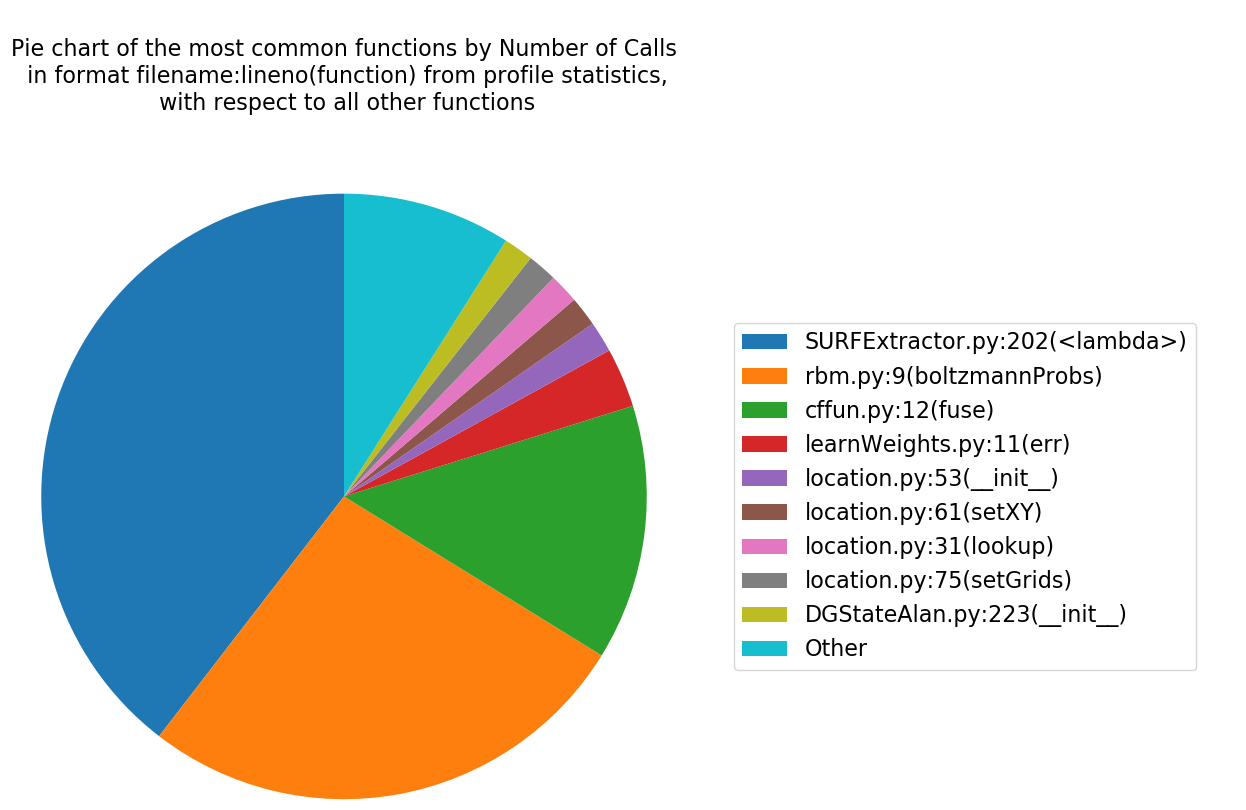
\includegraphics[width=0.7\textwidth]{figures/res_profiling/number_calls_cpu_crop.png}
    \caption{Number of calls for the CPU implementation of the model.}
    \label{fig:ncc}
\end{figure}

\begin{figure}
    \centering
    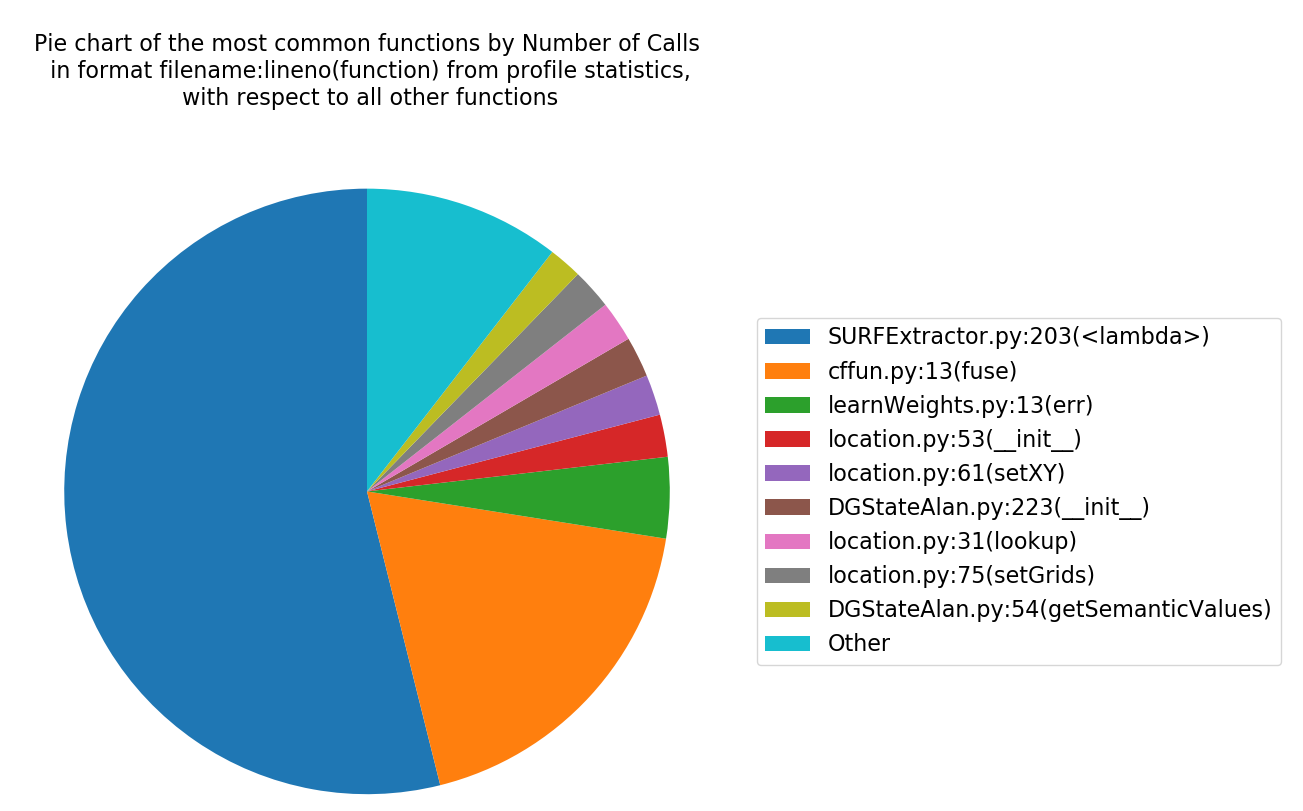
\includegraphics[width=0.7\textwidth]{figures/res_profiling/number_calls_gpu_crop.png}
    \caption{Number of calls for the GPU implementation of the model.}
    \label{fig:ncg}
\end{figure}

In contrast, profiling the Tensorflow version (\figureref{fig:ncg}) shows the lambda function from SURFExtractor taking a larger proportion of the total number of calls.
This is likely due to the usage of the \mono{tf.function} decorator optimisation.
The decorator converts the function into an optimised Tensorflow data call graph, which is loaded into the memory of the GPU at runtime.



Tensorflow processes the calls to the function such that the profiler only records the first time each call to \mono{boltzmannProbs} is hit, as opposed to everytime.
The \mono{cffun\#fuse} function has approximately the same amount of calls, and can probably be reduced by applying the \mono{tf.function} decorator.
Finally the \mono{learnWeights\#err} function has a constant number of calls across both implementations as it is not affected by the randomness of the model.


\subsection{Total time}

The more interesting profiling results come from the total time spent executing the function, excluding calls to other functions.
Initially the main functions that take the most time are the \mono{learn} function of the \mono{learnWeights} module, the \mono{boltzmannProbs} function of the \mono{rbm} module and the \mono{fuse} function of \mono{cffun} module as seen in \figureref{fig:ttc}.

After applying the parallel refactoring, the \mono{learnWeights\#learn} function takes a larger proportion of the overall time taken, as seen in \figureref{fig:ttg}.
The \mono{cffun\#fuse} function also has an increase in the proportion of time taken.
However, given that the overall time taken increases with a small amount of nodes, it indicates that there may be an underlying algorithmic problem which causes this behaviour.

\picturesque{figures/res_profiling/tot_time_cpu_crop.png}{Total time for function calls for the CPU implementation of the model.}{fig:ttc}

\picturesque{figures/res_profiling/tot_time_gpu_crop.png}{Total time for function calls for the GPU implementation of the model.}{fig:ttg}


In addition, the \mono{boltzmannProbs} function appears to have a large reduction in time taken.
However this is likely due to the \mono{tf.function} decorator function mapping the original function to a data call graph that runs purely on the GPU, which the Python profiler does not have access to.
This can be seen when using the line profiler on the \mono{boltzmannProbs} function.

%insert listing or similar thing depicting the output of line profiler, with full excerpt in an appendix.
\coderef{profiling:line_boltzmann} shows the results of profiling the \mono{boltzmannProbs} function line by line. 
It can be seen that the main bottleneck is the multiplication of the inputs and weights, taking approximately 60\% of the overall time.
This is likely due to the asynchronous nature of matrix multiplication, which is applied across a given dimension of the inputs. 


\begin{minipage}{\linewidth}
\begin{lstlisting}[caption=Line by line profiling of the rbm\#boltzmannProbs function in eager execution mode, label=profiling:line_boltzmann]
Total time: 237.186 s
Function: boltzmannProbs at line 9

Line #      Hits         Time  Per Hit   % Time  Line Contents
==============================================================
     9                                           @profile
    10                                           #@tf.function
    11                                           def boltzmannProbs(W, x, axis=0):      # RETURNS THE PROBABILITY OF A NODE BEING ON
    12    252240  143312866.0    568.2     60.4      mult = tf.tensordot(W, x, axis)
    13    252240   12193753.0     48.3      5.1      squeezed = tf.squeeze(mult)
    14    252240    6917896.0     27.4      2.9      E_on  = -squeezed       #penalty is the negative of the reward (just to make it look like energy
    15    252240   20604441.0     81.7      8.7      E_off = 0.0*E_on
    16    252240   13057317.0     51.8      5.5      Q_on = tf.math.exp(-E_on)       #as energy is negated, we have e^(reward)
    17    252240   12601996.0     50.0      5.3      Q_off = tf.math.exp(-E_off)
    18    252240   28258157.0    112.0     11.9      P_on = Q_on / (Q_on + Q_off)
    19    252240     239234.0      0.9      0.1      return P_on
\end{lstlisting}
\end{minipage}





\subsection{Unit tests}
\label{subsec:unittest}
{
A big problem with creating and improving software is that it is likely to break.
This is especially true when refactoring to speed up the code.
This is due to changes in underlying implementation creating side effects in the code.
These side effects cause the code to break, and if left unchecked increases the technical debt, which accrues as a natural part of the software development life-cycle.

\begin{minipage}{\linewidth}
\begin{lstlisting}[caption=Example unit to be tested, label=code:unit, language=python]
def boltzmannProbs(W, x, axis=0):
    """
    :param W: Input Weight Matrix
    :param x: Input Vector Matrix
    :param axis: Axis of contraction
    :return: activation probabilities
    """
    reward = tf.tensordot(W, x, axis)
    E_on  = tf.negative(reward)
    E_off = 0.0*E_on
    Q_on = tf.math.exp(-E_on)
    Q_off = tf.math.exp(-E_off)
    P_on = tf.math.divide(Q_on, tf.math.add(Q_on, Q_off))
    return P_on
\end{lstlisting}
\end{minipage}

Unit tests are a method of both reducing technical debt and ensuring that behaviour remains the same.
This is because the tests are used to verify behaviour after refactoring a unit.
A unit can be considered any functional object, however we define a unit as a custom function in the code.
An example of a unit can be seen in \coderef{code:unit}.
}



{
A test is a wrapper function that provides known inputs to the unit and checks the output of the unit against a known output.
The check is done via an assert statement.
An assert statement fails if the values that the assertion is checking do not match.
We define a test function as a singular concept on the unit being tested.
This allows us to understand the nature of the unit for that concept.
It also reduces confusion on what a given test is meant to do.
This reduces technical debt as future developers are not having to figure out what the 
purpose of a given test is, which increases productivity.
An example of a test can be seen in \coderef{code:test}
}



\begin{minipage}{\linewidth}
\begin{lstlisting}[caption=Example test for a unit, label=code:test, language=python]
def test_rbm_small():
    input_weights = np.array([[.1, .2], [.3, .4]])
    input_vector = np.array([.5, .6])
    calculated_results = rbm.boltzmannProbs(input_weights, input_vector)
    actual_results = np.array([0.54239794, 0.5962827])
    assert_almost_equal(calculated_results, actual_results,
                            err_msg="[BoltzmannProbs] Calculated results are not equal to actual results to 7 decimal places.")
\end{lstlisting}
\end{minipage}

{
%A big problem with the improvement of software is that it breaks when you change it. You are trying to speed it up but u change its functionality.   [introduce a problem]
%[sets you up to describe a solution]
%Units tests are an amazing way to fix this problem.  
%what is a unit test? 
%    what is a unit?
%        a function?  a class?  a file ?
%    what is a test?
%        one call of a unit? many calls of a unit?
%            many calls with a similar theme?
%        Used for testing how functions handle inputs and whether actual behaviour is what we expect.
%                using assertions
%                    say what is an assertion
%        show code examples  
%    martin fowler defined unit test as ...
 
 }      


\subsubsection{Test Driven Development and HC-UCPF}
Test Driven Development is a method of developing software that focuses on writing tests before writing code.
This allows the developer to write valid code the first time round, and does not need to spend long hours debugging the code.
This works well for new projects.
However our project involves refactoring an existing project.
Thus we can not follow test driven development to the letter.
But we can use the approach of test driven development as part of the refactoring process.
This means we write our tests and ensure that the existing code passes them.
This also has the benefit of helping to understand the purpose of the code.

By refactoring code in this manner, it helps with the process of debugging.
This is due to being able to pass the system inputs to the tests, and seeing what is causing the error.
Furthermore, from our definition of the unit test, we can obtain a hierarchical approach to debugging.
This is due to each of our functions being units, and invoking other functional units within our system.

For example, the function \verb|learn| in learnWeights.py\footnote{Found at \url{https://github.com/A-Yakkus/hclearn/blob/msc2020/learnWeights.py\#L16}} invokes the \verb|boltzmannProbs| function in rbm.py\footnote{Found at \url{https://github.com/A-Yakkus/hclearn/blob/msc2020/rbm.py\#L9}}.
If an error occurs during the learn function with respect to the \mono{boltzmannProbs} function, we can pause execution of the learn function and run the current inputs through our tests to find where the erroneous behaviour occurs.
Once we understand the erroneous behaviour, it can be considered trivial to fix it.
This would then allow successive invocations of the system to run without encountering the error. 

    % (though disputed by other people x y and z in these ways..)
    % what they do:
    %     they assure us that each unit works
    %     that allows us to try changing a unit
    %             eg to optimise
    %     it also allows delta debugging:
    %         hierarchy of unit tests
    %         find a bug by looking at red/green and homeing in
    %     what this is great
    %         saving tons of time! instant bug detection and localistion
    % TDD: write tests first
    % Refactoring: fowler's approach: how to optimise other peoples code  (vs TDDm is different)
    %     % Our case has it different as we already have functions implemented.
    % Parallel debugging:
    %   parallel is especially important use case here
    %         [NB we already told the reader about parallel techs, so we can refer to that now]
    %   new big idea here -- using fowler refactors to make parallel debugging tolerable !  is  big deal.



\subsection{Refactoring with Unit Tests}

Unit tests are traditionally used for the creation of software, as they are designed to help a developer create software.
This is because you can define the expected behaviour of a function and work to that definition.
However they can also be used in conjunction with profiling for speeding up known functions via refactoring.
This is because we can write the tests for a function that is causing the bottleneck from profiling.
We can then develop a new version of the function with Tensorflow, using these tests to preserve behaviour.

% As mentioned above, technical debt is created as part of the software development life-cycle.
% Technical debt is where software uses a quick lazy approach to code creation over properly developed code.
% In test driven development, technical debt occurs from developing the software without using tests.
% Refactoring can be used to reduce the technical debt created by developing a project.
% As an existing project, the HC-UCPF has technical debt.
% This indicates that refactoring will help reduce the overall technical debt.

% What is technical debt? 
% How is it created?

% What is refactoring?
% Why does it solve technical debt?

% Who is Fowler?
% What are his ideas?
% Why are they a good approach to refactoring?


A prominent figure in the field of refactoring is Martin Fowler.
Fowler describes unit testing as being situational, with a unit referring to an agreed upon identifier, such as a function, class or object, and a test referring to a fast, low-level implementation of the unit, focusing on a small part of the system ~\citep{fowlerUnit2014}.

Fowler suggests a hat-based approach to refactoring.
This means that as a developer, you would wear different metaphorical hats depending on the job.
Whilst wearing a particular hat, you purely focus on that job.
This reduces the chance of getting confused on what you are doing when working on the code.

% How does this relate to our project?
% \begin{itemize}
%     \item create unit tests to help understand what is going on with the code
%     \item implement new version for chosen parallel lib
%     \item integrate into system
%     \item full details in section 3.1
% \end{itemize}
% Fowler's Keynote speeches are the star here, namely the hat system. Our hats are testing (for unit tests), creation (for new tf code), integration (for implementing functions into system), ?system analysis (for delving into the namespace at specific points in execution/call stack and understanding what is going on)?

For our project, we are refactoring the model to allow for parallel execution of the learning process via unit testing.
This will also have the effect of making the learning easier to understand moving forward.
Hence we are reducing the technical debt of the project.
This allows us to create a number of hats for the different tasks, as follows:
\begin{itemize}
    \item A hat for the creation of unit tests.
    \item A hat for the development of parallel functions using Tensorflow.
    \item A hat for managing the integration of the parallel functions into the overall system.
\end{itemize}
% \noteAttention{What do these hats do?}
These hats can help guide the development of the project.
By developing the project in this way, we can control the scope of the refactoring, and keep it focused on the learning process, rather than the setup or evaluation.

Using the unit tests as a base for our refactoring is useful as it allows for faster system analysis in the event of a crash.
This is because the stack trace displayed when a crash occurs usually identifies the line that caused the crash.
This relies on the developer understanding the system to know how to fix it.

However our hierarchical approach to creating the unit tests reduces the amount of knowledge required.
This is because the inputs can be retrieved from a breakpoint in the debugging process, and then transferred to being inputs to a test script.
This test script then runs the unit tests on all functions and nested functions within that get invoked from the crash causing line.
Thus the overall time needed to fix the crash gets reduced as the unit tests identify how the crash is caused, making it easier to fix.
Furthermore, by reducing the amount of knowledge needed to understand the system at the onset of a project in this manner, we are able to curb the growth of future technical debt that the system may obtain.
% Why is this approach good for this method?
% \begin{itemize}
%     \item Allows for faster system analysis/debugging
%     \begin{itemize}
%         \item when code errors we get stack trace
%         \item stack trace usually identifies where problem is.
%         \item having unit tests for the identified problem makes it easier to identify problem and fix
%     \end{itemize}
%     \item reduces future technical debt
%     \begin{itemize}
%         \item functions often grow in scope
%         \item this allows for a trigger for when function is doing too much
%         \item KISS principle
%     \end{itemize}
% \end{itemize}



% We have only considered serial programming for refactoring
% however we are moving to a parallel approach
% this makes the software run asynchronously
% which makes it harder to identify where a problem lies

% This can be solved using unit tests in the fowler approach
% we can use the tests with inputs being the workgroups of the kernel launches
% This allows us to identify which workgroup is causing the problem.
% By identifying the problem input, we can work backwards through the software to find the first mutation which leads to the error.

